\ifx \allfiles \undefined
\documentclass[12pt,a4paper,oneside]{report}

%% === CJK 套件 ===
\usepackage{CJKutf8,CJKnumb}                 % 中文套件
%% === AMS 標準套件 ===
\usepackage{amsmath,amsfonts,amssymb,amsthm} % 數學符號
%% === ===
\usepackage{algorithm}
\usepackage{listings}                        % 程式碼
%% === TikZ 套件 ===
\usepackage{tikz,tkz-graph,tkz-berge}        % 繪圖
\usepackage{multicol}
%% == ==
\usepackage[unicode]{hyperref}
\usepackage{xcolor}
\hypersetup{
    colorlinks,
    linkcolor={blue!100!black},
    citecolor={blue!75!black},
    urlcolor={blue!50!black}
}
%% == 調整設定 ==
\usepackage{enumitem}                           % 修改 enumerate, item
\usepackage{bbding}
\usepackage{titletoc,titlesec,imakeidx}
%% == ==
\usepackage{newfloat}
\usepackage{caption,subcaption}
\usepackage{xkeyval,xargs}
\usepackage{ulem}
\usepackage{import}

%% === 設定 C++ 格式 ===
\lstset{%
  language=C++,             % 設定語言
  %% === 空白, tab 相關 ===
  tabsize=2,                % 設定 tab = 多少空白
  %showspaces=true,          % 設定是否標示空白
  %showtabs=true,            % 設定是否標示 tab
  %tab=\rightarrowfill,      % 設定 tab 樣式
  %% === 行數相關 ===
  numbers=left,             % 行數標示位置
  stepnumber=1,             % 每隔幾行標示行數
  numberstyle=\tiny,
  %breaklines=true,          % 設定斷行
  %% === 顏色設定 ===
  basicstyle=\ttfamily,
  keywordstyle=\color{blue}\ttfamily,
  stringstyle=\color{red!50!brown}\ttfamily,
  commentstyle=\color{green!50!black}\ttfamily,
  %identifierstyle=\color{black}\ttfamily,
  emphstyle=\color{purple}\ttfamily,
  extendedchars=false,
  texcl=true,
  moredelim=[l][\color{magenta}]{\#},
  captionpos=b,
  %% === 其他 ===
  %frame=single
}

% ===============================================
%
%  設定頁面格式
%
% ===============================================
%% === 設定頁面格式 ===
%\hoffset         = 10pt                      % 水平位移,預設為 0pt
\voffset         = -15pt                     % 垂直位移,預設為 0pt
\oddsidemargin   = 0pt                       % 預設為 31pt
%\topmargin       = 20pt                      % 預設為 20pt
%\headheight      = 12pt                      % header 的高度,預設為 12pt
%\headsep         = 25pt                      % header 和 body 的距離,預設為 25pt
\textheight      = 620pt                     % body 內文部分的高度,預設為 592pt
\textwidth       = 450pt                     % body 內文部分的寬度,預設為 390pt
%\marginparsep    = 10pt                      % margin note 和 body 的距離,預設為 10pt
%\marginparwidth  = 35pt                      % margin note 的寬度,預設為 35pt
%\footskip        = 30pt                      % footer 高度 + footer 和 body 的距離,預設為 30pt

%% ==  ==
\DeclareFloatingEnvironment[fileext=frm,placement={!ht},name=Frame]{code}
\captionsetup[code]{labelfont=bf}

\makeindex

\linespread{1.14}

\begin{document}
\begin{CJK}{UTF8}{bkai}

\subimport{../config/}{document-config.tex}

\fi

\providecommandx*{\Mat}[3][1=A,2=m,3=n]{%
  \ensuremath{{#1}_{{#2}\times{#3}}}}

\chapter{線性結構}

\section{陣列 (Array)}

\paragraph{}大家對陣列都不陌生,抽象意義上,陣列就是一群\textbf{有關聯}的元素排成的\textbf{序列 (Sequence)},這個序列可以是一維的,也可以是二維以上,二維以上的陣列看來不像是序列,反而像是矩陣 (二維時) 或是一大堆數字整齊地堆在一起 (二維以上),因此陣列又有另外的稱呼叫做\textbf{數組 (Array)}。

\begin{figure}[h!]
  \centering
  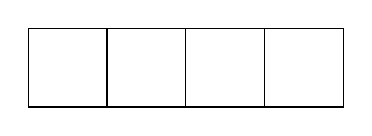
\begin{tikzpicture}
  \draw (0,0) rectangle (1,1);
  \draw (1,0) rectangle (2,1);
  \draw (2,0) rectangle (3,1);
  \draw (3,0) rectangle (4,1);
  \end{tikzpicture}
  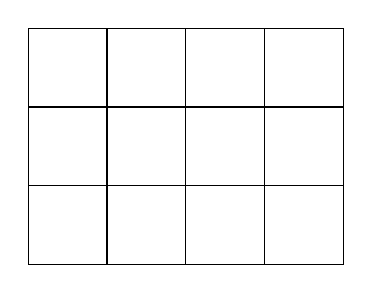
\begin{tikzpicture}
  \draw (0,0) rectangle (1,1);
  \draw (1,0) rectangle (2,1);
  \draw (2,0) rectangle (3,1);
  \draw (3,0) rectangle (4,1);
  \draw (0,1) rectangle (1,2);
  \draw (1,1) rectangle (2,2);
  \draw (2,1) rectangle (3,2);
  \draw (3,1) rectangle (4,2);
  \draw (0,2) rectangle (1,3);
  \draw (1,2) rectangle (2,3);
  \draw (2,2) rectangle (3,3);
  \draw (3,2) rectangle (4,3);
  \end{tikzpicture}
  \caption{一維陣列(左)和二維陣列(右),或稱數組、矩陣}
  \label{fig:array:1-dim-and-2-dim}
\end{figure}

\paragraph{}因為陣列是「\textbf{關係上連續}」的元素所形成的序列,所以實際上,我們有兩種作法:
\begin{enumerate}
  \item 第一種是讓他真的在實際的記憶體上連續,這就是我們常用的陣列;
  \item 第二種,我們不管他是不是在記憶體上連續,模擬連續的情形,這種又有一個名稱叫做\textbf{鏈結串列 (Linked list)},如下圖 4.2:
\end{enumerate}

\section{大數 (Big Number)}

\paragraph{}有些時候,我們可能會存不下數字,這些存不下的數字我們稱為\textbf{大數 (Big number)}。例如整數 (integer) 最多只能存到 $2^{32}-1$ (無號),長整數 (long integer) 最多只能存到 $2^{64}-1$ (無號),不管是任何的程式語言,都有他的限制,那麼們要怎樣儲存一個連最強大的資料型態都不能儲存的數呢?

\paragraph{}我們用陣列來模擬。如果現在給你一個數字 $1234567890$,我們用陣列將數字一位一位儲存,如下圖 4.3。

\subsection{大數加法與減法}
\paragraph{}我們知道怎麼儲存後,接著我們要知道怎麼運算,很簡單,就像我們\textbf{小學的加減法}一般,將個位數對齊、十位數對齊、百位數對齊、$\cdots$ 以此類推,全部加起來就可以囉。當然,回憶一下我們小學的時候,算加減法一定會注意\textbf{進位和借位 (carry)},因此我們的程式也要自己去模擬進位和借位,不同的是,我們做加減法時可以先不用處理進位,等到後來再一口氣進位。時間複雜度為 $O(n)$。

\paragraph{}以下為大數加法的虛擬碼:

\subimport{../problem/}{04-linear-list-bigint-add-and-sub.tex}

\subsection{大數乘法}

\subimport{../problem/}{04-linear-list-bigint-multi.tex}

\subsection{大數除法}

\subimport{../problem/}{04-linear-list-bigint-div.tex}

\subsection{更有效率的大數}

\subimport{../problem/}{04-linear-list-bigint-more-efficient.tex}

\section{矩陣 (Matrix)}
\subsection{定義}

\paragraph{}矩陣就是二維陣列,若說一維陣列是一個由 $n$ 個元素排成一列的結構,那麼矩陣可以看做是有 $m$ 個一維陣列並排,每個一維陣列有 $n$ 個元素排成一列。
\paragraph{}通常我們用\textbf{英文字母大寫}來稱呼矩陣,如下圖是矩陣 $A$,裡面所有元素形成一個二維陣列,其中下圖的 $a[1,1]$、$a[1,2]$、$a[1,3]$、$\cdots$、$a[1,n]$,$n$ 個元素形成一個\textbf{列 (row)},$a[1,1]$、$a[1,2]$、$\cdots$ 等等叫做第一列,$a[2,1]$、$a[2,2]$、$\cdots$ 等等叫做第二列,以此類推;同樣地,$a[1,1]$、$a[2,1]$、$\cdots$、$a[m,1]$,$m$ 個元素形成一個\textbf{行 (column)},$a[1,1]$、$a[2,1]$、$\cdots$、$a[m,1]$ 就是第一行。二維陣列有兩個註標,通常來說,第一個註標表示列,第二個註標表示行,例如第 $i$ 列第 $j$ 行的元素就是 $a[i,j]$。

\paragraph{}如果要描述一個矩陣的大小,我們就看他有幾列幾行,一個有 $m$ 列 $n$ 行的矩陣被稱為一個 $m\times{n}$ 矩陣,記為 \textbf{$\Mat$}。如果 $m=n$ 的話,我們稱為\textbf{方陣},或是 $n$ 階矩陣,例如一個 $3\times{3}$ 的矩陣我們可以稱他為 $3$ 階矩陣。

\paragraph{}矩陣其他的性質眾多,以下只介紹高中才會接觸到的範圍,其他的東西,有興趣的讀者可以參考大學的一門課程「\textbf{線性代數}」。

\subimport{../problem/}{04-linear-list-matrix-def.tex}

\subsection{矩陣加法與減法}

\paragraph{}矩陣加法的規則很簡單,假設現在有兩個矩陣 $\Mat$ 和 $\Mat[B]$,兩個矩陣的\textbf{大小必須一樣},則
\begin{align*}
A+B=a[i,j]+b[i,j]
\end{align*}
,意即 A 與 B 每個\textbf{對應元素}相加;矩陣減法和加法類似,$A-B=a[i,j]-b[i,j]$,代表 A 和 B 矩陣相減。舉例,甲國與乙國生產汽車和稻米,將去年的產量和今年的產量做成下面兩表:

\paragraph{}假設我們要計算\textbf{兩年間},兩國所有汽車和稻米的總產量,那麼就會應用到矩陣加法:

\paragraph{}我們可以很清楚地從圖 4.13 看到矩陣加法的運算方式,如果矩陣的大小不同,也就直接代表兩個矩陣的資料沒有對應,因此不同大小的矩陣無法相加似乎挺自然的(?),如果兩個矩陣大小一樣,但是裡面的資料屬性不同呢?以圖 4.14 來說:

\paragraph{}丙國不生產汽車,取而代之的是生產麵粉和稻米,那麼這個矩陣可以和前面兩個甲國和乙國的矩陣相加嘛?

\paragraph{}就矩陣加法而言,它是可以相加的 (因為矩陣大小相同),矩陣加法只是提供一個\textbf{抽象的運算概念},並無法表示兩個矩陣相加的實際意涵,就如同我們知道 $2+3=5$,但要是 $2$ 顆蘋果加上 $3$ 台汽車呢?讀者可以思考一下。

\subsection{矩陣乘法}

\paragraph{}接著我們看看矩陣乘法,不少讀者可能會認為矩陣乘法的運算複雜,但只要抓住它核心的思想,那麼矩陣乘法應是很好理解的。

\paragraph{}假設現在有兩個矩陣 $\Mat[A][m][r]$ 和 $\Mat[B][r][n]$ \textbf{(注意矩陣大小)},做矩陣乘法後的矩陣為 $\Mat[C][m][n]$ \textbf{(注意矩陣大小)},運算規則為:
\begin{align*}
A\times{B}=C=c[i,j]=\sum^{r}_{k=1}{a[i,k]\times{b[k,j]}}
\end{align*}

\paragraph{}看起來非常複雜?我們一步一步來分析矩陣乘法。首先,我們\textbf{再三}要注意的是,矩陣乘法的 $A$、$B$ \textbf{唯一的限制}--$A$ 的行數要和 $B$ 的列數\textbf{相同},圖 4.15 表示了這個條件。

\paragraph{}從圖 4.15 可以看到,矩陣乘法的方向,當我們的矩陣相乘時,前面的矩陣\textbf{橫著走},後面的矩陣\textbf{順著往下走},假設是 $A$ 矩陣的第 $i$ 列、$B$ 矩陣的第 $j$ 行,運算公式告訴我們這兩個相乘後會產生
\begin{align*}
c[i,j] &= a[i,1]\times{b[1,j]}+a[i,2]\times{b[2,j]}+\cdots{}+a[i,k]\times{b[k,j]}+\cdots{}+a[i,r]\times{b[r, j]}
\end{align*}
,每個 $a[i,k]$ 一定會和 $b[k,j]$ 相乘,因此 $A$ 的行數和 $B$ 的列數一定要\textbf{一樣}才能做乘法,否則會沒有對應。

\paragraph{}如果照著規則走的話,那麼最後產生的矩陣就會是一個 $m\times{n}$ 的矩陣:因為 $A$ 是 $m\times{r}$ 的矩陣,而 $B$ 是 $r\times{n}$ 的矩陣,其中我們在做乘法的過程中,我們會把 $A$ 矩陣第 $i$ 列和 $B$ 矩陣第 $j$ 行的 $r$ 個數相乘並相加,最後變成 $C$ 矩陣的一個數--$c[i,j]$。

\paragraph{}因為 $A$ 矩陣有 $m$ 列,$C$ 矩陣也會有 $m$ 列;同理,因為 $B$ 矩陣有 $n$ 行,所以 $C$ 矩陣也依然會有 $n$ 行,總而言之,$C$ 矩陣就是個 $m\times{n}$ 的矩陣。

\subimport{../problem/}{04-linear-list-matrix-multi.tex}

\subsection{單位元素與反元素}

\subimport{../problem/}{04-linear-list-matrix-identity-inverse-element.tex}

\subsection{行列式}
\subsection{反矩陣}

\subimport{../problem/}{04-linear-list-matrix-inverse-matrix.tex}

\subsection{高斯消去法}

\subimport{../problem/}{04-linear-list-matrix-gauss.tex}

\subsection{01 矩陣與運算}

\subimport{../problem/}{04-linear-list-matrix-01-matrix.tex}

\section{鏈結串列 (Linked-List)}
\subsection{鏈結串列實作 (Implementation)}
\subsection{更多變形}
\section{堆疊 (Stack)}
\subsection{括號匹配}
\subsection{前序、中序、後序表達式}
\subsection{排隊視線問題}
\section{佇列 (Queue)}
\subsection{佇列 (Queue)}
\subsection{優先佇列 (Priority Queue)}

\ifx \allfiles \undefined

\printindex[noun]
\clearpage

\end{CJK}
\end{document}

\fi